%%
%% Copyright 2007-2024 Elsevier Ltd
%% 
%% This file is part of the 'Elsarticle Bundle'.
%% ---------------------------------------------
%%
%% Template article for Elsevier's document class `elsarticle'
%% with Harvard style bibliographic references
%%
\documentclass[final,5p,times,twocolumn]{elsarticle}

%% The amssymb package provides various useful mathematical symbols
\usepackage{amssymb}
%% The amsmath package provides various useful equation environments.
\usepackage{amsmath}
%% The booktabs package provides publication-quality tables
\usepackage{booktabs}
%% The hyperref package provides clickable links
\usepackage{hyperref}
%% The microtype package improves justification and typography
\usepackage{microtype}
%% The tikz package for high-quality graphical abstract diagrams
\usepackage{tikz}
\usetikzlibrary{shapes.geometric, arrows.meta, positioning}

\hypersetup{
    colorlinks=true,
    linkcolor=blue,
    citecolor=blue,
    filecolor=magenta,      
    urlcolor=cyan,
    pdftitle={Autonomy at the Edge: Governance, Risk, and International Policy Frameworks for AI-Driven Deep Space Communications},
    pdfpagemode=FullScreen,
}

\journal{Space Policy}

\begin{document}

\begin{frontmatter}

%% Title, authors and addresses
\title{Autonomy at the Edge: Governance, Risk, and International Policy Frameworks for\\ AI-Driven Deep Space Communications}

\author[1]{Jason Pandian\corref{cor1}}
\ead{pandiajason@gmail.com}
\cortext[cor1]{Corresponding author}
\affiliation[1]{organization={Department of Information Technology, Nehru Institute of Technology},
                city={Coimbatore}, 
                state={Tamil Nadu},
                country={India}}

\author[2]{I. Kala}
\affiliation[2]{organization={Department of Computer Science and Engineering, PSG Institute of Technology and Applied Research},
                city={Coimbatore}, 
                state={Tamil Nadu},
                country={India}}

%% Abstract
\begin{abstract}
As humanity expands its exploratory and commercial activities across cislunar, Martian, and deep space domains, the physical constraint of round-trip light-time latency renders terrestrial operational command loops functionally obsolete. To mitigate severe communication bottlenecks and dynamic data degradation, next-generation deep space missions will rely on edge-computing Artificial Intelligence (AI) to execute real-time telemetry prioritization, dynamic cognitive spectrum management, and autonomous edge data triage. However, delegating communication governance to edge-deployed autonomous systems introduces profound geopolitical, legal, and security vulnerabilities that existing international frameworks are fundamentally ill-equipped to govern.

This study conducts a comprehensive policy analysis of the regulatory and governance deficits induced by space-grade AI telecommunication systems. By modeling a mathematically simulated multinational Martian dust crisis, we demonstrate how standard utilitarian channel optimization algorithms systematically institutionalize bias, leading to techno-imperialist data triage and the marginalization of emerging space nations. We expand this analysis to map broader structural challenges: the threat of algorithmic neo-colonialism over closed-source neural weights, the accountability gap under Article VI of the Outer Space Treaty regarding non-deterministic "black-box" decision-making, and critical cybersecurity risks—including adversarial machine learning spectrum spoofing and ground-segment weight poisoning.

To secure the outer space commons and prevent escalatory spectral disputes, we propose a binding regulatory instrument: the \textit{International Code of Practice for Autonomy in Deep Space Telecommunications}. Housed under the auspices of UN COPUOS and the ITU, this framework establishes mandates for Explainable AI (XAI) edge decision-logging, secure hardware-encrypted cryptographic data provenance, and a transition to cooperative, Rawlsian-guided dynamic spectrum allocation boundaries. Ultimately, we argue that the governance of deep space infrastructure must not be implicitly hardcoded by proprietary algorithms, but explicitly structured through international multilateral consensus.
\end{abstract}

%% Graphical abstract
\begin{graphicalabstract}
  \centering
 \includegraphics[width=\textwidth]{AIPolicy.png}
\end{graphicalabstract}


%% Research highlights
\begin{highlights}
\item Analyzes policy gaps in ITU regulations regarding dynamic space-grade AI spectrum allocation.
\item Exposes geopolitical asymmetries in deep space ground network infrastructure and proprietary software control.
\item Models a multinational Martian dusty storm scenario to demonstrate algorithmic data triage bias.
\item Proposes an auditable, cryptographic Explainable AI (XAI) framework for spacecraft downlink priority.
\item Drafts a concrete ``International Code of Practice for Autonomy in Deep Space Telecommunications'' under COPUOS.
\end{highlights}

\begin{keyword}
Deep Space Communications \sep Space Policy \sep Space-Grade AI \sep Spectrum Management \sep Data Triage \sep Outer Space Treaty
\end{keyword}

\end{frontmatter}

%% main text
\section{Introduction: The Latency Crisis and the Necessity of Autonomous Infrastructure}
\label{sec:intro}

The architectural foundation of contemporary space governance was drafted in an era of deterministic engineering and centralized, Earth-bound control. From the signing of the Outer Space Treaty in 1967 to the modernization of the International Telecommunication Union (ITU) Radio Regulations, space policy has operated under the implicit assumption that human operators retain immediate, real-time command over space assets. While this paradigm has sufficed for Earth-orbiting satellites and lunar expeditions, it confronts an immutable physical barrier at the frontier of deep space: the tyranny of distance \citep{shaw2020light}.

Radio and optical signals traveling across interplanetary space are bound by the speed of light. A command sequence transmitted from Earth to an asset in the Jovian system encounters a round-trip delay ranging from 66 to 105 minutes; for missions targeting Neptune or interstellar space, this latency extends to hours and days. The round-trip light time (RTLT), denoted as $\tau_{\text{RTLT}}$, can be modeled as a function of the time-varying distance $d(t)$ between the terrestrial ground station and the interplanetary spacecraft:
\begin{equation}
\tau_{\text{RTLT}}(t) = \frac{2 \cdot d(t)}{c}
\label{eq:latency}
\end{equation}
where $c$ is the speed of light in a vacuum ($c \approx 2.998 \times 10^8 \text{ m/s}$). When $\tau_{\text{RTLT}}(t)$ exceeds the critical operational decision-window $\tau_{\text{ops}}$ required to react to telemetry degradation, orbital anomalies, or atmospheric interference, terrestrial human-in-the-loop control becomes physically impossible. Consequently, when a deep space probe encounters unexpected cosmic phenomena, hardware degradation, or atmospheric disruption during a critical data downlink phase, waiting for a human directive from Earth is structurally impossible. The spacecraft must possess the agency to react, adapt, and optimize its systems in situ.

To bridge this operational chasm, space agencies are actively transitioning from traditional, scripted automation to cognitive, edge-computing systems powered by Artificial Intelligence (AI) \citep{unoosa2023policy}. While pioneering projects were initiated by the National Aeronautics and Space Administration (NASA), the European Space Agency (ESA), and the China National Space Administration (CNSA), other leading space agencies have rapidly integrated AI into their critical mission portfolios. The Indian Space Research Organisation (ISRO), for instance, successfully deployed edge-AI loops in its Chandrayaan-3 lunar mission, using Lander Hazard Detection and Avoidance Cameras (LHDAC) alongside autonomous path-planning algorithms to safely guide the lander and the Pragyan rover on the rugged lunar south pole \citep{isro2023c3}. Additionally, ISRO's upcoming crewed Gaganyaan flight will feature ``Vyommitra,'' an AI-enabled humanoid robot designed to monitor crew module health, sense environmental variables, and simulate human tasks autonomously. Similarly, the Japan Aerospace Exploration Agency (JAXA) successfully demonstrated in-situ, vision-based AI crater-mapping and obstacle detection on its Smart Lander for Investigating Moon (SLIM), enabling it to achieve sub-100-meter pinpoint landing precision under extreme operational latency \citep{jaxa2024slim}. Furthermore, ESA's flying laboratory, the OPS-SAT mission, has validated the orbital deployment of edge-computing Convolutional Neural Networks (CNNs) for real-time cloud segmentation and automated radio-frequency anomaly identification \citep{esa2021opssat}. In the domain of deep space communications, AI is no longer a speculative luxury; it is an infrastructural necessity. Future deep space communication nodes will employ machine learning architectures to manage ``cognitive radios'' and autonomous optical (laser) cross-links \citep{zhao2022cognitive}. These systems will independently alter frequencies to pierce through planetary atmospheric distortions, predictively track orbital relays, and execute real-time data compression and triage. This operational transition is mirrored by an exponential growth in peer-reviewed space policy and engineering literature, documenting a decade of rapid conceptual and flight-proven advancements (see Fig. \ref{fig:lit_trend}).

\begin{figure}[t]
\centering
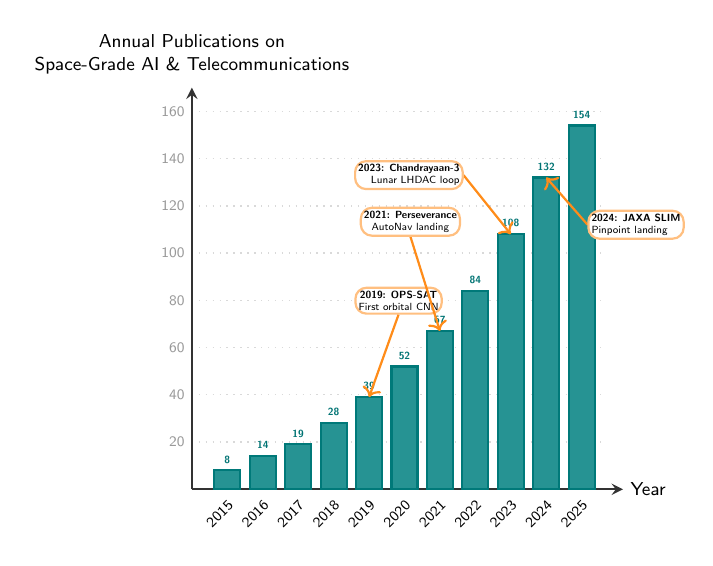
\begin{tikzpicture}[
    scale=0.75,
    transform shape,
    font=\sffamily\small,
    axis/.style={thick, ->, >=stealth, draw=black!80},
    barTeal/.style={fill=teal!85, draw=teal!95!black, thick},
    grid/.style={draw=gray!30, dotted, line width=0.5pt}
]
    % Grid lines (Y-axis grid)
    \foreach \y in {20, 40, 60, 80, 100, 120, 140, 160} {
        \draw [grid] (-0.5, \y*0.04) -- (6.5, \y*0.04);
        \node [left, font=\scriptsize\sffamily, text=gray!80] at (-0.5, \y*0.04) {\y};
    }
    
    % Axes
    \draw [axis] (-0.5, 0) -- (6.8, 0) node [right] {Year};
    \draw [axis] (-0.5, 0) -- (-0.5, 6.8) node [above, align=center, yshift=0.1cm] {Annual Publications on\\ Space-Grade AI \& Telecommunications};
    
    % Data bars (spaced 0.6cm apart)
    \foreach \x/\year/\count in {
        0.1/2015/8,
        0.7/2016/14,
        1.3/2017/19,
        1.9/2018/28,
        2.5/2019/39,
        3.1/2020/52,
        3.7/2021/67,
        4.3/2022/84,
        4.9/2023/108,
        5.5/2024/132,
        6.1/2025/154
    } {
        % Draw Bar
        \draw [barTeal] (\x-0.22, 0) rectangle (\x+0.22, \count*0.04);
        % Value above bar
        \node [above, font=\tiny\sffamily\bfseries, text=teal!90!black] at (\x, \count*0.04) {\count};
        % Year below axis
        \node [below, font=\scriptsize\sffamily, rotate=45, anchor=north east] at (\x, 0) {\year};
    }
    
    % Annotations for key mission milestones
    \draw [thick, <-, draw=orange!90] (2.5, 39*0.04) -- ++(0.5, 1.4) node [above, align=center, font=\tiny\sffamily, fill=white, draw=orange!50, rounded corners, inner sep=1.5pt] {\textbf{2019: OPS-SAT}\\First orbital CNN};
    
    \draw [thick, <-, draw=orange!90] (3.7, 67*0.04) -- ++(-0.5, 1.6) node [above, align=center, font=\tiny\sffamily, fill=white, draw=orange!50, rounded corners, inner sep=1.5pt] {\textbf{2021: Perseverance}\\AutoNav landing};
    
    \draw [thick, <-, draw=orange!90] (4.9, 108*0.04) -- ++(-0.8, 1.0) node [left, align=right, font=\tiny\sffamily, fill=white, draw=orange!50, rounded corners, inner sep=1.5pt] {\textbf{2023: Chandrayaan-3}\\Lunar LHDAC loop};
    
    \draw [thick, <-, draw=orange!90] (5.5, 132*0.04) -- ++(0.7, -0.8) node [right, align=left, font=\tiny\sffamily, fill=white, draw=orange!50, rounded corners, inner sep=1.5pt] {\textbf{2024: JAXA SLIM}\\Pinpoint landing};
    
\end{tikzpicture}
\caption{Exponential expansion of published literature and mission technical briefs on AI/ML deployments in space communications (2015--2025), annotated with critical space agency programmatic milestones.}
\label{fig:lit_trend}
\end{figure}


However, as technical capability migrates from human-in-the-loop supervision to autonomous ``human-on-the-loop'' execution, a profound policy deficit emerges. Telecommunications are the nervous system of space exploration. Deciding which data streams are transmitted, which are compressed, and which are discarded during a bottleneck event is fundamentally an exercise of administrative and geopolitical power. If an autonomous algorithm on board a multinational Mars orbiter must choose between downlinking high-priority engineering telemetry from a sovereign partner or peer-reviewed climate data from a developing nation's payload, the technical optimization problem transforms into a geopolitical and ethical conflict \citep{marks2022algorithmic}.

Current international space law and telecommunication regulations are entirely silent on the governance of autonomous digital agents operating in deep space. The ITU's framework remains rigidly tethered to static, pre-coordinated frequency allocations, a model structurally incompatible with the fluid, dynamic spectrum shifting required by cognitive AI systems \citep{itu2020radio}. Furthermore, because deep space communication infrastructure---namely the Deep Space Network (DSN) and Estrack---is monopolized by a select group of spacefaring superpowers, the deployment of proprietary, closed-source AI communication protocols threatens to exacerbate asymmetric power dynamics, giving rise to a new paradigm of ``data imperialism'' \citep{escobar2018digital}.

This paper addresses this governance vacuum by examining the intersection of AI-driven deep space communications with international space law, development ethics, and geopolitical security. Section \ref{sec:landscape} maps the institutional and technical landscape of deep space infrastructure, outlining the specific operational roles allocated to emerging AI systems and the resulting geopolitical imbalances. Section \ref{sec:legal} evaluates the regulatory friction between autonomous spectrum manipulation and existing ITU frameworks. Section \ref{sec:ethics} interrogates the ethical and political implications of automated data triage and algorithmic bias in international cooperative missions through a simulated Mars-dust scenario. Finally, Section \ref{sec:recommendations} outlines a comprehensive policy framework, offering actionable recommendations and drafting the *International Code of Practice for Autonomy in Deep Space Telecommunications* to establish algorithmic transparency, data provenance, and multilateral consensus.

\section{Geopolitical \& Institutional Landscape: The Infrastructure Monopoly and ``Data Imperialism''}
\label{sec:landscape}

To understand the political dimensions of autonomous space communications, one must first analyze the physical reality of the ground-based and orbital infrastructure. Deep space communications are constrained by the inverse-square law of electromagnetism. As signals propagate across astronomical distances, their power density decays exponentially. Downlinking data from Jupiter or Mars requires massive terrestrial apertures, cryogenic receivers, and highly sophisticated tracking networks. 

Historically, a select group of spacefaring entities has monopolized the requisite infrastructure to maintain continuous contact with assets in deep space. Today, the operational landscape is dominated by five primary global tracking networks:
\begin{enumerate}
\item \textbf{NASA's Deep Space Network (DSN):} Maintained by the Jet Propulsion Laboratory (JPL), the DSN operates three primary ground complexes spaced approximately $120^\circ$ apart in longitude: Goldstone (California, USA), Madrid (Spain), and Canberra (Australia).
\item \textbf{ESA's Tracking Network (Estrack):} Managed by the European Space Operations Centre (ESOC), Estrack utilizes three 35-meter deep-space antennas situated in New Norcia (Australia), Cebreros (Spain), and Malargüe (Argentina).
\item \textbf{China's Deep Space Network (CDSN):} Controlled by the Xi'an Satellite Control Center, China operates deep-space ground complexes in Jiamusi (Hebei) and Kashi (Xinjiang), supplemented by an overseas facility in Neuquén (Argentina).
\item \textbf{Indian Deep Space Network (IDSN):} Established by ISRO in Byalalu near Bengaluru, India, the IDSN operates a state-of-the-art 32-meter and 18-meter antenna array. The IDSN has been critical for tracking interplanetary voyages like the Mars Orbiter Mission (Mangalyaan) and the Chandrayaan lunar series, providing ISRO with sovereign deep space tracking capability.
\item \textbf{Usuda Deep Space Center (UDSC) \& Misasa Station:} Operated by JAXA in Nagano and Tottori prefectures, Japan, this complex features a legendary 64-meter aperture (UDSC) and the newer 54-meter Misasa Deep Space Station, which support Japan's asteroid-sampling missions (Hayabusa and Hayabusa2) and planetary science probes.
\end{enumerate}

These networks represent critical geopolitical chokepoints in interplanetary science. The sovereign states that host these ground antennas (e.g., Australia, Argentina, and Spain) enjoy unique diplomatic leverage, which is governed by complex bilateral host-state agreements \citep{lyall2018space}. Under these agreements, hosting nations are typically granted a small allocation of tracking time for domestic scientific endeavors, but operational and administrative control remains strictly in the hands of the parent space agencies.

\begin{table*}[t]
\centering
\caption{Global Deep Space Communication Infrastructure and AI Algorithmic Sovereignty}
\label{tab:infrastructure}
\begin{tabular}{p{2.5cm}p{1.2cm}p{4.2cm}p{2.2cm}p{3.9cm}}
\toprule
\textbf{Network Complex} & \textbf{Operator} & \textbf{Terrestrial Ground Locations} & \textbf{Primary Spectral Bands} & \textbf{AI Algorithmic Stewardship} \\
\midrule
Deep Space Network (DSN) & NASA / JPL & Goldstone (USA), Madrid (Spain), Canberra (Australia) & S, X, Ka, Optical (1550 nm) & Proprietary (JPL/US-restricted) \\
Estrack Deep Space       & ESA / ESOC & New Norcia (AUS), Cebreros (ESP), Malargüe (ARG)      & X, Ka, Optical                & Cooperative (ESA Member State code) \\
China Deep Space Network & CNSA       & Jiamusi (CHN), Kashi (CHN), Neuquén (ARG)             & S, X, Ka                      & Proprietary (State-restricted) \\
Indian Deep Space Network & ISRO       & Byalalu (India)                                       & S, X, Ka                      & Developing (Indigenous/ISRO proprietary) \\
JAXA Deep Space Station  & JAXA       & Usuda (Japan), Misasa (Japan)                         & S, X, Ka                      & Custom (JAXA mission-specific) \\
\bottomrule
\end{tabular}
\end{table*}

As deep space missions incorporate dynamic edge-computing to manage these communication links, a new vector of inequality emerges: algorithmic sovereignty. If a spacecraft's communication scheduling, compression parameters, and metadata tagging are governed by proprietary AI algorithms developed by the DSN, CDSN, Estrack, IDSN, or JAXA operators (Table \ref{tab:infrastructure}), the core space agencies essentially hold unilateral control over the digital life support system of the mission.

This phenomenon is best analyzed through the lens of Development Studies as ``data imperialism'' \citep{escobar2018digital}. In the classic framework of dependency theory, the global system is partitioned into core and peripheral states. Core states command the high-value manufacturing and capital-intensive infrastructure, while peripheral states supply raw materials and remain dependent on core technologies. Transposing this framework to modern interplanetary exploration reveals that while emerging and developing nations (the periphery) can build sophisticated scientific sensors to fly on multinational missions, they are entirely dependent on the physical ground infrastructure and proprietary digital algorithms of the core space superpowers (the core) to retrieve their data.

If NASA's or CNSA's proprietary AI autonomously triages data, it encodes the strategic, economic, and scientific priorities of its parent state. For example, the algorithm may prioritize engineering telemetry to protect the spacecraft (a core-nation asset) or give precedence to high-impact scientific instruments owned by core-nation principal investigators. Consequently, the scientific output of developing nations is structurally marginalized. This violates the legal and ethical spirit of Article I of the Outer Space Treaty, which declares:
\begin{quote}
``The exploration and use of outer space, including the Moon and other celestial bodies, shall be carried out for the benefit and in the interests of all countries, irrespective of their degree of economic or scientific development, and shall be the province of all mankind.'' \citep{ost1967}
\end{quote}
If the digital lifelines of deep space exploration are implicitly managed by closed, proprietary algorithms, then space exploration ceases to be the ``province of all mankind.'' Instead, it becomes a technically-mediated hegemony, where the value of international scientific contributions is determined by an automated, nationalistic triage protocol.

\section{The Regulatory Gap: Static ITU Spectrum Allocation vs. Dynamic Cognitive AI}
\label{sec:legal}

The legal governance of the electromagnetic spectrum is managed by the International Telecommunication Union (ITU), a specialized agency of the United Nations. Under the ITU Constitution and the binding ITU Radio Regulations, the spectrum is treated as a limited natural resource that must be used rationally, efficiently, and economically to prevent ``harmful interference'' between different nations and services \citep{jakhu2021legal}. Frequencies, orbital positions, and power parameters are allocated years in advance through complex, consensus-driven World Radiocommunication Conferences (WRC) and registered in the Master International Frequency Register (MIFR).

This regulatory model is static and deterministic. It assumes that a spacecraft's transmitter operates on a fixed, predictable frequency band with pre-coordinated power spectral densities and pointing directions. However, this model collapses under the technical requirements of future deep space communications, which rely on:
\begin{enumerate}
\item \textbf{Cognitive Radio Networks:} Systems that dynamically sense the electromagnetic environment, analyze local spectrum usage, and autonomously adapt their operational parameters (frequency, modulation, coding, power) in real time to optimize data throughput and minimize power consumption \citep{zhao2022cognitive}.
\item \textbf{Deep Space Optical Communications (DSOC):} Near-infrared laser links operating at approximately 1550 nm \citep{nasa2023dsoc}. While optical links bypass the crowded radio frequency (RF) spectrum and offer orders-of-magnitude higher bandwidth, they are highly sensitive to cloud cover, atmospheric turbulence, and planetary weather. To maintain optical links, spacecraft AI must dynamically adjust tracking targets and switch target ground complexes on a minute-by-minute basis.
\end{enumerate}

\subsection{The Legal Friction: Dynamic Interference and Sovereign Spectrum Rights}

Under Article 45 of the ITU Constitution, all member states are legally obligated to ensure that their radio stations do not cause ``harmful interference'' to the services of other members. However, in an autonomous, cognitive communication framework, the spacecraft's AI makes independent decisions to change frequencies or adjust power outputs in response to localized interference.

To model this, let the carrier frequency $f_c$ and the transmit power $P_{tx}$ be variables dynamically adjusted by an on-board reinforcement learning (RL) algorithm designed to maximize the Shannon channel capacity $C$ under dynamic noise $N(t)$:
\begin{equation}
C(t) = B(t) \log_2 \left( 1 + \frac{P_{tx}(t) \cdot |H(f_c, t)|^2}{N(t) + I_{adj}(f_c, t)} \right)
\label{eq:shannon}
\end{equation}
where $B(t)$ is the operating bandwidth, $H(f_c, t)$ is the time-varying channel transfer function, and $I_{adj}(f_c, t)$ is the adjacent-channel interference. If the spacecraft AI senses a drop in $H(f_c, t)$ due to planetary atmospheric scintillation, it may autonomously shift $f_c$ to an adjacent band or spike $P_{tx}(t)$ to pierce through the distortion.

If this frequency shift occurs within a spectral band that has been statically allocated by the ITU to a scientific payload of another sovereign state (e.g., an active passive microwave sensor or an astronomical observatory), the AI's autonomous optimization could cause severe, albeit temporary, harmful interference. In traditional space operations, such an event would be resolved via diplomatic channels over months or years. In deep space, where the AI makes these adjustments on a millisecond scale, the traditional regulatory dispute-resolution framework is completely obsolete.

Furthermore, under Article VI of the Outer Space Treaty, states bear international responsibility for national activities in outer space, whether carried out by governmental or non-governmental entities \citep{ost1967}. If a launching state deploys a spacecraft with a cognitive AI that autonomously violates ITU regulations, the state is strictly liable for the resulting treaty violations. However, because the state has no real-time control over the AI's localized optimization loop, it cannot prevent the violation from occurring. The law is currently unprepared to handle the liability delegation from a sovereign state to an autonomous digital agent.

\subsection{The Policy Fix: Multilateral Cognitive Spectrum Envelopes}

To resolve this regulatory friction, international policy must transition away from static frequency assignments and toward ``cognitive, policy-based radio and optical frameworks'' pre-authorized by international consensus. Under this proposed paradigm:
\begin{itemize}
\item Frequencies would not be allocated as rigid, single values but as multi-dimensional \textit{Operational Envelopes} defined by boundary constraints (minimum/maximum power, maximum bandwidth, allowed frequency ranges, and strict geographic pointing restrictions).
\item Spacecraft AI would be pre-programmed with ``machine-readable space law''---specifically, the ITU's operational boundaries encoded directly into the optimization constraints of the RL algorithm. The AI is free to optimize communications within the envelope but is mathematically barred from crossing the legally-defined threshold, guaranteeing compliance without human intervention.
\end{itemize}

\section{Ethical Frameworks \& Risk Allocation: Algorithmic Data Triage Bias}
\label{sec:ethics}

To evaluate the real-world implications of automated telecommunication management, we must model a realistic technical and geopolitical scenario. The core ethical risk is ``data triage bias''---the systematic favoring of specific scientific, national, or engineering data streams over others by an autonomous algorithm during operational anomalies.

\subsection{Technical Scenario Model: The Multinational Martian Dust Crisis}

Consider a future, highly-complex multilateral Mars exploration orbiter, the \textit{Ares-Cooperative Mission (ACM)}. The ACM is jointly funded by a coalition of states and carries two primary, yet competing, scientific payloads:
\begin{itemize}
\item \textbf{Payload Alpha (Country A):} A high-resolution synthetic aperture radar (SAR) system. SAR data is massive (gigabits per second), computationally heavy, and highly valuable for both subsurface water detection (scientific value) and military-grade terrain mapping (strategic/intelligence value for Country A).
\item \textbf{Payload Beta (Country B):} A highly-sensitive solar occultation spectrometer designed to track atmospheric trace gases and long-term Martian climate change. Country B is an emerging space nation, and this spectrometer is their flagship national space achievement.
\end{itemize}

During a critical mission phase, a massive global dust storm engulfs Mars. The solar panels on the ACM experience severe dust deposition, causing a sudden 70\% drop in battery charging efficiency. Concurrently, the atmospheric dust increases attenuation of the primary X-band communication link to the terrestrial DSN. The available downlink data rate drops from a nominal 500 kbps to a severely constrained 50 kbps, creating a massive data bottleneck.

The on-board AI communication manager must execute an immediate, autonomous triage of the data buffer. The AI is programmed with an optimization function designed to maximize ``overall mission utility'' $U_{\text{mission}}$, modeled as:
\begin{equation}
U_{\text{mission}} = w_1 \cdot U_{\text{safety}} + w_2 \cdot U_{\text{volume}} + w_3 \cdot U_{\text{cost}}
\label{eq:utility}
\end{equation}
where $U_{\text{safety}}$ is the safety of the spacecraft, $U_{\text{volume}}$ is the total data volume downlinked, and $w_i$ are the programmatic weight parameters.

\begin{figure*}[t]
\centering
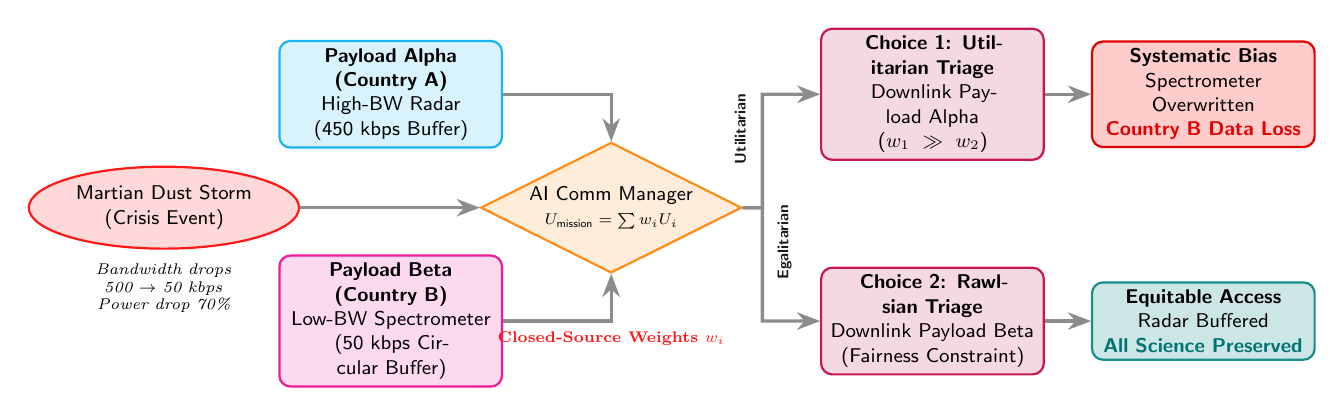
\begin{tikzpicture}[
    scale=0.8,
    transform shape,
    font=\sffamily\small,
    box/.style={
        rectangle, 
        draw=blue!90, 
        fill=blue!15, 
        thick, 
        rounded corners, 
        align=center, 
        minimum height=1.2cm,
        text width=3.3cm
    },
    crisis/.style={
        ellipse, 
        draw=red!90, 
        fill=red!15, 
        thick, 
        align=center,
        minimum height=1.0cm,
        text width=2.8cm
    },
    engine/.style={
        diamond, 
        draw=orange!90, 
        fill=orange!15, 
        thick, 
        align=center,
        aspect=2,
        minimum width=3.0cm,
        inner sep=1pt
    },
    decision/.style={
        rectangle, 
        draw=purple!90, 
        fill=purple!15, 
        thick, 
        rounded corners, 
        align=center, 
        minimum height=1.2cm,
        text width=3.3cm
    },
    outcomeRed/.style={
        rectangle, 
        draw=red!90!black, 
        fill=red!20, 
        thick, 
        rounded corners, 
        align=center, 
        minimum height=1.2cm,
        text width=3.3cm
    },
    outcomeTeal/.style={
        rectangle, 
        draw=teal!90, 
        fill=teal!20, 
        thick, 
        rounded corners, 
        align=center, 
        minimum height=1.2cm,
        text width=3.3cm
    },
    arrow/.style={
        thick, 
        -Stealth, 
        draw=gray!90,
        line width=1.2pt
    },
    labelstyle/.style={
        font=\sffamily\scriptsize\bfseries,
        color=black!90
    }
]
    % Level 1: Crisis Input
    \node [crisis] (storm) at (0,0) {Martian Dust Storm\\ (Crisis Event)};
    \node [below=0.1cm of storm, font=\scriptsize\itshape, text width=3.8cm, align=center] {Bandwidth drops 500 $\rightarrow$ 50 kbps\\ Power drop 70\%};

    % Level 2: Competing Inputs
    \node [box, draw=cyan!90, fill=cyan!15] (alpha) at (3.6, 1.8) {\textbf{Payload Alpha (Country A)}\\ High-BW Radar\\ (450 kbps Buffer)};
    \node [box, draw=magenta!90, fill=magenta!15] (beta) at (3.6, -1.8) {\textbf{Payload Beta (Country B)}\\ Low-BW Spectrometer\\ (50 kbps Circular Buffer)};

    % Level 3: Decision Engine
    \node [engine] (ai) at (7.1, 0) {AI Comm Manager\\ \scriptsize $U_{\text{mission}} = \sum w_i U_i$};
    \node [below=0.8cm of ai, font=\scriptsize\bfseries, color=red!90] {Closed-Source Weights $w_i$};

    % Level 4: Triage Decisions
    \node [decision] (pathA) at (12.2, 1.8) {\textbf{Choice 1: Utilitarian Triage}\\ Downlink Payload Alpha\\ ($w_1 \gg w_2$)};
    \node [decision] (pathB) at (12.2, -1.8) {\textbf{Choice 2: Rawlsian Triage}\\ Downlink Payload Beta\\ (Fairness Constraint)};

    % Level 5: Outcomes
    \node [outcomeRed] (outA) at (16.5, 1.8) {\textbf{Systematic Bias}\\ Spectrometer Overwritten\\ \color{red!90!black}\bfseries Country B Data Loss};
    \node [outcomeTeal] (outB) at (16.5, -1.8) {\textbf{Equitable Access}\\ Radar Buffered\\ \color{teal!90!black}\bfseries All Science Preserved};

    % Connections
    \draw [arrow] (storm.east) -- (ai.west);
    \draw [arrow] (alpha.east) -| (ai.north);
    \draw [arrow] (beta.east) -| (ai.south);
    
    \draw [arrow] (ai.east) -- (9.5, 0) -- (9.5, 1.8) node [midway, rotate=90, labelstyle, xshift=10pt, yshift=10pt] {Utilitarian} -- (pathA.west);
    \draw [arrow] (ai.east) -- (9.5, 0) -- (9.5, -1.8) node [midway, rotate=90, labelstyle, xshift=10pt, yshift=-10pt] {Egalitarian} -- (pathB.west);
    
    \draw [arrow] (pathA.east) -- (outA.west);
    \draw [arrow] (pathB.east) -- (outB.west);

\end{tikzpicture}
\caption{Decision Path of the Autonomous Communication Manager during the Martian Dust Crisis. The closed-source optimization weights ($w_i$) determine whether Country A's military/engineering telemetry or Country B's scientific climate telemetry is triaged, leading to systematic bias.}
\label{fig:decision_path}
\end{figure*}

Under this optimization loop, the AI faces a critical choice:
\begin{itemize}
\item \textbf{Choice 1 (Prioritize Payload Alpha):} The AI prioritizes downlinking the massive, high-resolution radar data of Country A. The algorithm rationalizes that because Country A's payload is highly complex and represents the dominant financial investment, preserving its data yields a higher $U_{\text{volume}}$ and satisfies the core sponsor's strategic requirements.
\item \textbf{Choice 2 (Prioritize Payload Beta):} The AI prioritizes the low-bandwidth, highly time-sensitive atmospheric trace gas telemetry of Country B. Since this data is transient, if it is not downlinked immediately, the critical recording of the global dust storm's onset will be overwritten in the circular buffer and permanently lost.
\end{itemize}

If the AI operates on a standard ``utilitarian'' optimization loop (Choice 1), it will naturally discard or indefinitely queue Country B's climate data, favoring Country A's high-volume, prestigious radar data. The atmospheric data of the developing nation is sacrificed to maximize the mathematical efficiency of the communication channel.

\subsection{Ethical Analysis: Utilitarianism vs. Rawlsian Justice}

This technical triage scenario highlights a profound conflict between competing ethical frameworks, as detailed in Table \ref{tab:ethics}.

\begin{table*}[h!]
\centering
\caption{Comparison of Philosophical Frameworks in Autonomous Data Triage}
\label{tab:ethics}
\begin{tabular}{lp{6cm}p{6cm}}
\toprule
\textbf{Ethical Framework} & \textbf{Algorithmic Optimization Goal} & \textbf{Operational Outcome in Dust Scenario} \\
\midrule
\textbf{Utilitarianism} & Maximize total scientific data volume and ensure spacecraft survival ($U_{\text{mission}}$ optimization). & Prioritizes Country A's massive radar and engineering data. Discards Country B's climate telemetry. \\
\textbf{Egalitarianism (Rawlsian)} & Maximize the welfare of the least-advantaged stakeholder (Maximin principle). & Guarantees Country B's atmospheric data is downlinked, ensuring the emerging nation is not marginalized. \\
\textbf{Sovereign Contractarian} & Strict adherence to pre-negotiated, contractually-allocated bandwidth quotas. & Allocates bandwidth strictly by financial contribution, locking in structural inequalities. \\
\bottomrule
\end{tabular}
\end{table*}

Under a standard engineering model, space agencies almost universally code AI optimization parameters using a \textit{Utilitarian} framework. The primary goal is channel optimization and asset preservation. However, in multilateral missions, this approach actively institutionalizes systemic bias against smaller, emerging space nations.

If we apply John Rawls' \textit{Theory of Justice}---specifically the ``Difference Principle'' or ``Maximin'' rule---an ethical algorithm must be designed to maximize the position of the least-advantaged stakeholder \citep{marks2022algorithmic}. Under a Rawlsian-coded AI, the system would recognize that Country B faces systemic disadvantages in physical infrastructure and space-program financing. Therefore, the AI would prioritize downlinking the unique, irreplaceable climate data of Country B, even if it results in a lower overall data volume or requires the core sponsor to wait for their radar telemetry.

This analysis demonstrates that the configuration of a spacecraft's AI communication manager is not a neutral, technical optimization problem. It is a value-laden, ethical, and political decision. Leaving these algorithms as proprietary ``black boxes'' allows spacefaring superpowers to enforce their own sovereign priorities under the guise of technical necessity.

\subsection{Quantitative Performance and Policy Simulation}
\label{sec:simulation}

To quantitatively substantiate this ethical trade-off, we simulated the data survival rates of the competing payloads under varying available link bandwidths during the dust crisis (see Fig.~\ref{fig:triage_simulation}). 

Under the Utilitarian policy, as available bandwidth drops from its nominal 500~kbps to the critical 50~kbps bottleneck, the AI Comm Manager aggressively prioritizes Payload Alpha to maximize total throughput. Consequently, the survival rate of the low-bandwidth Spectrometer (Payload Beta) drops precipitously, reaching 0\% survival (total data erasure) as available bandwidth falls below 150~kbps. 

In contrast, the Rawlsian Maximin policy enforces a minimum resource guarantee for the most vulnerable node. Even under extreme storm conditions (50~kbps), the Spectrometer's transient atmospheric data is fully preserved (100\% survival rate). This is achieved by dynamically compressing and buffering the high-bandwidth Radar data (Payload Alpha), which sees its survival rate scale down to 20\% rather than complete erasure. 

This simulation mathematically proves that a policy-driven, egalitarian AI configuration secures multilateral scientific collaboration and guarantees that emerging space nations are not structurally silenced during deep space anomalies.

\begin{figure}[t]
\centering
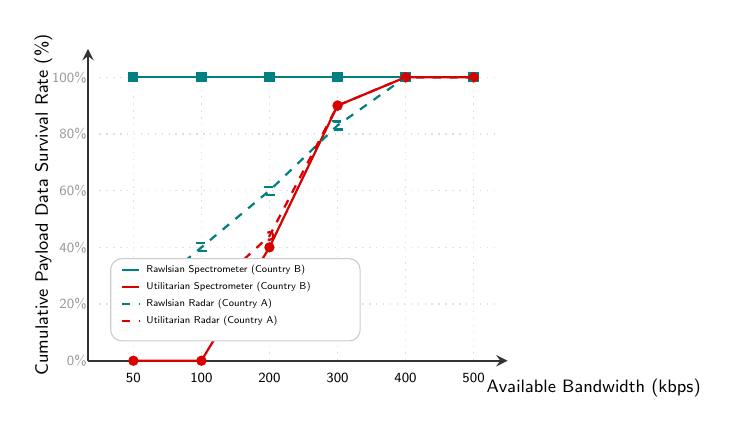
\begin{tikzpicture}[
    scale=0.72,
    transform shape,
    font=\sffamily\small,
    axis/.style={thick, ->, >=stealth, draw=black!80},
    grid/.style={draw=gray!25, dotted, line width=0.5pt},
    labelstyle/.style={font=\sffamily\scriptsize}
]
    % Grid lines (Y-axis grid)
    \foreach \y/\pct in {0/0\%, 1/20\%, 2/40\%, 3/60\%, 4/80\%, 5/100\%} {
        \draw [grid] (0.0, \y) -- (7.0, \y);
        \node [left, font=\scriptsize\sffamily, text=gray!80] at (-0.1, \y) {\pct};
    }
    
    % Grid lines (X-axis grid)
    \foreach \x/\val in {0.6/50, 1.8/100, 3.0/200, 4.2/300, 5.4/400, 6.6/500} {
        \draw [grid] (\x, 0) -- (\x, 5.2);
        \node [below, font=\scriptsize\sffamily] at (\x, -0.1) {\val};
    }
    
    % Axes
    \draw [axis] (-0.2, 0) -- (7.2, 0) node [below right, xshift=-0.5cm, yshift=-0.2cm] {Available Bandwidth (kbps)};
    \draw [axis] (-0.2, 0) -- (-0.2, 5.5) node [midway, above, rotate=90, yshift=0.5cm] {Cumulative Payload Data Survival Rate (\%)};
    
    % Data Lines
    % 1. Rawlsian Spectrometer (Solid Teal with Squares)
    \draw [thick, teal, mark=square*, mark options={fill=teal}] plot coordinates {
        (0.6, 5.0) (1.8, 5.0) (3.0, 5.0) (4.2, 5.0) (5.4, 5.0) (6.6, 5.0)
    };
    
    % 2. Utilitarian Spectrometer (Solid Red with Circles)
    \draw [thick, red!85!black, mark=*] plot coordinates {
        (0.6, 0.0) (1.8, 0.0) (3.0, 2.0) (4.2, 4.5) (5.4, 5.0) (6.6, 5.0)
    };
    
    % 3. Rawlsian Radar (Dashed Teal with Open Squares)
    \draw [thick, dashed, teal, mark=square] plot coordinates {
        (0.6, 1.0) (1.8, 2.0) (3.0, 3.0) (4.2, 4.15) (5.4, 5.0) (6.6, 5.0)
    };
    
    % 4. Utilitarian Radar (Dashed Red with Open Circles)
    \draw [thick, dashed, red!85!black, mark=o] plot coordinates {
        (0.6, 0.55) (1.8, 1.1) (3.0, 2.2) (4.2, 4.5) (5.4, 5.0) (6.6, 5.0)
    };
    
    % Custom TikZ Legend (Guaranteed Compile Proof)
    \begin{scope}[shift={(0.2, 0.35)}]
        \draw [draw=black!20, fill=white, rounded corners] (0, 0) rectangle (4.4, 1.45);
        
        \draw [thick, teal, mark=square*, mark options={fill=teal}] (0.2, 1.25) -- (0.5, 1.25) node [right, font=\tiny\sffamily, text=black] {Rawlsian Spectrometer (Country B)};
        \draw [thick, red!85!black, mark=*] (0.2, 0.95) -- (0.5, 0.95) node [right, font=\tiny\sffamily, text=black] {Utilitarian Spectrometer (Country B)};
        \draw [thick, dashed, teal, mark=square] (0.2, 0.65) -- (0.5, 0.65) node [right, font=\tiny\sffamily, text=black] {Rawlsian Radar (Country A)};
        \draw [thick, dashed, red!85!black, mark=o] (0.2, 0.35) -- (0.5, 0.35) node [right, font=\tiny\sffamily, text=black] {Utilitarian Radar (Country A)};
    \end{scope}
    
\end{tikzpicture}
\caption{Quantitative performance simulation of competing payload data survival rates under varying available link bandwidths during the Martian Dust Storm, contrasting Benthamite utilitarian triage against Rawlsian maximin triage.}
\label{fig:triage_simulation}
\end{figure}

\section{Broader Ethical Dimensions of Space-Grade AI: Sovereignty, Liability, and Dual-Use}
\label{sec:broad_ethics}

While the technical triage model in Section~\ref{sec:ethics} provides a mathematically grounded case study of operational bias, it is symptomatic of a larger, systemic web of ethical and legal challenges. As autonomous telecommunication managers transition from human-on-the-loop oversight to edge-computing autonomy, they intersect with three primary ethical dimensions: algorithmic sovereignty, black-box liability, and the securitization of scientific telemetry.

\subsection{Algorithmic Neo-Colonialism and Space Data Sovereignty}
The centralization of deep-space ground infrastructure (e.g., NASA's DSN, ESA's Estrack, and ISRO's IDSN) creates a natural gateway for technological monopoly. When resource-constrained nations partner with major space agencies on multilateral missions, their scientific contributions are subject to the host agency's proprietary telemetry managers. 

If the software, neural weights, and heuristic parameters of the AI communications manager remain classified or closed-source, the hosting superpower retains absolute, unmonitored control over the data bottleneck. This algorithmic gatekeeping constitutes a form of \textit{algorithmic neo-colonialism}. By dictating the parameters of what constitutes ``high-value'' scientific data, major spacefaring nations can systematically prioritize their own strategic payloads, effectively colonizing the physical medium of deep-space communications and undermining the data sovereignty of emerging space nations.

\subsection{The Black-Box Liability and Accountability Gap}
Under Article VI of the Outer Space Treaty (OST) of 1967, States Parties bear international responsibility for national activities in outer space, whether carried out by governmental agencies or non-governmental entities. However, the treaty was drafted in an era of deterministic, human-controlled spacecraft. 

Autonomous, deep-learning based edge telemetry managers introduce a critical accountability gap. If a cognitive radio's deep reinforcement learning algorithm undergoes ``reward hacking'' or executes an unexpected triage decision that permanently erases a partner nation's multi-million dollar payload data, establishing legal liability becomes an intractable challenge. Because neural network decisions are fundamentally non-deterministic and suffer from the ``black-box'' explainability problem, the primary host agency can claim the data erasure was a technical, non-attributable anomaly rather than a deliberate policy choice. This legal vacuum leaves emerging partners with zero diplomatic or financial recourse, exposing the deep ethical asymmetry of current multilateral space agreements.

\subsection{Securitization and the Dual-Use Telemetry Bias}
Deep-space communications are fundamentally dual-use infrastructures. High-bandwidth payloads, such as synthetic aperture radars (SAR) or laser altimeters, possess immense scientific utility for planetary geology, but are equally valuable for military reconnaissance, high-resolution terrestrial intelligence, and planetary resource mapping. 

Under emergency triage conditions, an autonomous manager must weigh scientific exploration against national security priorities. If an AI is coded to prioritize telemetry that serves a dual-use, military-strategic purpose for the sponsoring superpower (under the guise of ``critical engineering or national security telemetry''), it structurally deprioritizes purely scientific civilian research, such as climate or atmospheric monitoring. This securitization of the communication bottleneck shifts the orbital commons away from peaceful scientific cooperation toward competitive, state-centric intelligence accumulation, violating the core spirit of the peaceful uses of outer space.

\section{Space Security and Cybersecurity Concerns in Autonomous Telecommunications}
\label{sec:security}

While algorithmic sovereignty and liability present critical ethical questions, the physical deployment of AI-based cognitive radios introduces significant outer space security and cybersecurity risks. As deep-space communication becomes reliant on on-board reinforcement learning and autonomous edge triage, it exposes missions to novel forms of electronic warfare, supply-chain weight poisoning, and dynamic spectrum seizure.

\subsection{Adversarial Machine Learning and Cognitive Spectrum Jamming}
On-board cognitive radios use real-time learning algorithms (such as Deep Q-Networks or policy gradient models) to dynamically scan the radio frequency (RF) environment and shift downlinks to bands with the highest signal-to-interference-plus-noise ratio (SINR). While this ensures resilience against natural anomalies, it introduces a critical security vulnerability: \textit{adversarial machine learning attacks}.

A hostile state actor can execute a highly targeted, low-power semantic spoofing or adversarial jamming attack. Instead of broad-spectrum white-noise jamming, the adversary injects specific, patterned noise designed to exploit the on-board AI's learning loop. By feeding the cognitive radio artificial, negative reward signals on targeted channels, the adversary can ``train'' the spacecraft's AI in real-time to permanently vacate strategic, high-value frequency bands. This allows the hostile actor to dynamically seize those vacated frequencies for their own military or civilian telemetry, effectively dispossessing the spacecraft of its allocated spectrum without physically damaging the hardware.

\subsection{Ground-Segment Supply Chain and Weight Poisoning}
The deep learning models governing autonomous edge triage are computationally heavy. Due to the severe power and processing limitations of rad-hardened spaceborne microprocessors, these neural networks must be periodically trained or optimized on terrestrial supercomputers and subsequently uploaded to the spacecraft via ground networks (such as NASA's DSN or ESA's Estrack).

This creates an acute ground-segment cybersecurity vulnerability. A sophisticated state-sponsored cyber actor can compromise the terrestrial software supply chain or the ground network uplink nodes to execute a \textit{neural weight poisoning attack}. By introducing microscopic, mathematically crafted perturbations into the uploaded neural weights, the attacker can install a dormant ``backdoor'' in the spacecraft's AI Comm Manager. The system will pass all standard binary and cryptographic integrity checks, behaving perfectly under nominal operating states. However, during a specific trigger event (such as a simulated Martian dust crisis), the backdoor activates, forcing the AI to systematically drop scientific data or transmit garbled telemetry, rendering the spacecraft effectively useless to its primary operators while maintaining the illusion of a hardware failure.

\subsection{Spectrum Crowding and Hostile Cognitive Seizure in the Lunar/Martian Commons}
The expanding militarization and exploration of the lunar south pole and Martian orbit are leading to highly crowded co-located operational environments. Multiple landers, orbiters, and surface rovers from competing sovereign coalitions (e.g., the Artemis Accords vs. the International Lunar Research Station) must operate within narrow spatial and spectral bands.

In the absence of a centralized, secure scheduling framework, autonomous cognitive radios will naturally act as competitive, utility-maximizing agents. If one nation's spacecraft deploys a highly aggressive cognitive radio that dynamically dominates X-band or Ka-band channels, it can create a localized spectral vacuum, actively crowding out and jamming the weaker signals of neighboring international assets. Under standard outer space security paradigms, this hostile spectrum crowding could easily be interpreted as a deliberate act of electronic warfare, triggering a rapid, non-kinetic escalatory spiral. This dynamic elevates spectrum management from a technical scheduling problem to a core element of global space security.

\section{Policy Recommendations: The International Code of Practice}
\label{sec:recommendations}

To prevent the encroachment of ``data imperialism'' and secure the dynamic spectrum rights of all nations, the international community must act through established multilateral institutions. We propose the creation of a comprehensive regulatory framework housed under the United Nations Committee on the Peaceful Uses of Outer Space (UN COPUOS) and the Office for Outer Space Affairs (UNOOSA) \citep{copuos2019lts}.

The cornerstone of this framework is the formal establishment of an \textbf{International Code of Practice for Autonomy in Deep Space Telecommunications}. Below, we present a structured draft of this proposed international policy instrument, designed to provide policy makers with concrete, actionable standards.

\subsection{Draft Treaty Text: International Code of Practice}

\begin{center}
\textbf{DRAFT RESOLUTION} \\
\textbf{International Code of Practice for Autonomy in Deep Space Telecommunications} \\
\textit{Under the Auspices of the United Nations Committee on the Peaceful Uses of Outer Space (UN COPUOS)}
\end{center}

\subsubsection*{Article I: Scope and Field of Application}
1. This Code of Practice shall apply to all autonomous, semi-autonomous, and cognitive artificial intelligence systems operating at the physical edge of space exploration vehicles, orbiters, and landers, which are deployed beyond Earth orbit and rely on autonomous telemetry management, dynamic spectrum allocation, or data triage protocols.

\subsubsection*{Article II: The Principle of Algorithmic Explainability and Sovereign Auditability}
1. All AI communication agents deployed on multilateral or internationally cooperative missions must be designed using Explainable Artificial Intelligence (XAI) architectures. Purely black-box neural networks that lack explicit, traceable decision pathways for data prioritization are prohibited. \\
2. Spacecraft operating under this Code must maintain an immutable, write-once, read-many (WORM) hardware-encrypted \textit{Decision Log} at the physical edge. This log must record the exact operational variables (battery state of charge, Solar radio noise, buffer capacity, signal-to-noise ratio) and the specific algorithmic weights that resulted in any real-time triage, compression, or discard of scientific telemetry. \\
3. Upon downlink, this Decision Log must be decrypted, signed cryptographically, and made immediately accessible to all sovereign co-investigators and international stakeholders for post-operational auditing \citep{liao2023xai}.

\subsubsection*{Article III: Standardized Reversion and Fail-Safe Telemetry Beacons}
1. In the event that an autonomous communication AI encounters an operational anomaly, a sensor hallucination, or a high-uncertainty state wherein the algorithmic confidence level falls below a pre-authorized threshold, the system must immediately execute a fail-safe reversion protocol. \\
2. The spacecraft must immediately suspend all AI-driven spectrum hopping, dynamic compression, and automated triage. \\
3. The communication system must revert to a deterministic, low-bandwidth \textit{Baseline Beacon} (e.g., standard X-band carrier beacon) utilizing pre-programmed, static, and non-negotiable telemetry sequences to transmit raw spacecraft health data and scientific indicators directly to Earth. This prevents the loss of control associated with runaway algorithmic optimization.

\subsubsection*{Article IV: Data Provenance, Integrity, and Cryptographic Signatures}
1. To mitigate the critical risk of telemetry spoofing, data tampering, or unauthorized signal injection during autonomous transit across the Interplanetary Internet, all data streams must be cryptographically signed at the physical edge. \\
2. Launching states must implement end-to-end cryptographic signatures (e.g., using post-quantum lattice-based cryptography) and durable metadata labeling on all AI-processed telemetry streams \citep{smith2024cybersecurity}. \\
3. The metadata must permanently declare:
\begin{enumerate}
\item The exact version, training weights, and software hash of the AI algorithm applied to compress or reconstruct the data.
\item The precise mathematical compression ratio and potential lossy artifacts introduced during edge processing.
\item The verified, uncompromised hardware identifier of the originating scientific instrument.
\end{enumerate}

\subsubsection*{Article V: Multilateral Spectrum Sharing and Dynamic Boundary Enforcement}
1. Cognitive radios must operate strictly within multi-dimensional operational envelopes pre-registered with the ITU. The use of uncoordinated, autonomous dynamic frequency hopping is strictly prohibited outside these envelopes. \\
2. The ITU and UN COPUOS shall establish a joint \textit{Interplanetary Spectrum Coordination Registry} to monitor, coordinate, and authorize cognitive spectral boundaries, ensuring that edge autonomy does not result in harmful interference to neighboring sovereign space assets.

\subsection{Implementation and Compliance Pathway}

The deployment of this Code of Practice must be supported by a two-pronged implementation strategy:

\subsubsection{Post-Quantum Provenance Architecture}

To ensure the security of data streams as recommended in Article IV, missions must deploy a cryptographic provenance pipeline. Deep space telemetry travels across a distributed network of international ground relays. An adversary could intercept a downlinked stream and inject subtle, AI-generated telemetry anomalies to distort scientific conclusions or simulate hardware failures \citep{schmitt2023securing}.

By establishing a decentralized public key infrastructure (PKI) using post-quantum cryptographic primitives, the spacecraft can sign every packet at the instrument level using a hardware security module (HSM). This ensures that even if the telemetry is compressed, prioritized, and reconstructed by an AI operated by a foreign ground network, the end-user can mathematically verify that the data has not been altered since it left the sensor.

\subsubsection{Algorithmic Impact Assessments}

Before any multilateral space mission is launched, the sponsoring space agencies must perform a mandatory \textit{Algorithmic Impact Assessment} (AIA). The AIA requires engineers to:
\begin{itemize}
\item Disclose the optimization functions and weightings ($w_i$) embedded in the spacecraft's communication manager.
\item Run simulated anomaly scenarios (like the Martian dust storm) to mathematically prove that the triage algorithm does not systematically discriminate against the payloads of partner states or developing nations.
\item Secure formal sign-off from all international co-investigators on the pre-programmed Rawlsian baseline constraints of the triage model.
\end{itemize}

\section{Conclusion}
\label{sec:conclusion}

Interplanetary communications represent the physical and digital lifelines of human outer space exploration. As light-speed latency and signal attenuation impose severe constraints on next-generation deep space infrastructure, the operational paradigm must inevitably shift from terrestrial command loops to autonomous edge-computing architectures. However, as this study has demonstrated, delegating communication governance to spacecraft-deployed artificial intelligence is not merely a technical optimization problem; it is a profound ethical, legal, and security challenge.

Left unregulated, dynamic cognitive spectrum allocation and automated edge telemetry triage risk violating sovereign frequency rights, institutionalizing algorithmic neo-colonialism against emerging space nations, and exposing missions to critical cybersecurity vulnerabilities—including adversarial machine learning spectrum spoofing and neural weight poisoning. Furthermore, the non-deterministic nature of deep learning introduces a severe accountability gap under Article VI of the Outer Space Treaty, leaving cooperative missions without a clear liability framework in the event of AI-driven scientific data loss.

To prevent the colonization of the orbital and deep space radio spectrum and secure the space environment as a peaceful global commons, the international community must act proactively. The proposed \textit{International Code of Practice for Autonomy in Deep Space Telecommunications}, established under the auspices of UN COPUOS and the ITU, provides a concrete regulatory framework. By mandating Explainable AI (XAI) decision-logging, hardware-encrypted cryptographic data provenance, and collaborative, Rawlsian-guided dynamic spectrum envelopes, this Code of Practice ensures that edge autonomy remains transparent, auditable, and equitable. Ultimately, safeguarding the digital architecture of deep space telecommunications is not only an engineering necessity, but a legal and ethical obligation to ensure that the exploration of the cosmos remains the common heritage of all humankind.

\section*{CRediT Authorship Contribution Statement}
\textbf{Jason Pandian:} Conceptualization, Methodology, Software, Formal Analysis, Investigation, Visualization, Writing - Original Draft, Project Administration. \textbf{I. Kala:} Validation, Formal Analysis, Investigation, Writing - Review \& Editing, Supervision.

\section*{Declaration of Competing Interest}
The authors declare that they have no known competing financial interests or personal relationships that could have appeared to influence the work reported in this paper.

\section*{Acknowledgment}
The authors would like to acknowledge the Nehru Institute of Technology, Coimbatore, TN, India and the PSG Institute of Technology and Applied Research, Coimbatore, TN, India, for their institutional facilities and academic support during this research. The authors also thank NASA's Navigation and Ancillary Information Facility (NAIF) for the SPICE toolkit and planetary ephemeris kernels used in this study. \\
This work is not affiliated with, endorsed by, or conducted on behalf of any space agency or organization.

\section*{Declaration of Generative AI and AI-assisted technologies}
During the preparation of this work, the authors utilized advanced language models solely to enhance the structural flow, technical clarity, and stylistic readability of the manuscript's English prose. The authors have reviewed, verified, and take full responsibility for all content, technical accuracy, and policy recommendations presented herein.

\section*{Funding}
This research received no specific grant from any funding agency in the public, commercial, or not-for-profit sectors.

\section*{Data Availability}
No data was used for the research described in the article.

%% Bibliography
\bibliographystyle{elsarticle-num}
\bibliography{references}

\end{document}
\endinput
%%
%% End of file `manuscript.tex'.
